%-----------------------------------------------------------------------------------------------
\makeatletter
\immediate\write18{datelog > \jobname.info} % site script for $(date '+%Y-%m-%d %Hh%Mm%Ss')
\makeatother
%-----------------------------------------------------------------------------------------------
%-----------------------------------------------------------------------------------------------
\usetheme{Copenhagen}
\usepackage{beamercolorthemeCNThermSci2}
\usefonttheme{serif}
%-----------------------------------------------------------------------------------------------

%-----------------------------------------------------------------------------------------------
%-----------------------------------------------------------------------------------------------
\usetheme{Copenhagen}
\usepackage{beamercolorthemeUTF2}
\usefonttheme{serif}
%-----------------------------------------------------------------------------------------------
\usepackage[utf8]{inputenc}
\usepackage[greek,french,english,brazil]{babel} % last becomes the active one
\usepackage{pslatex}
\usepackage{amssymb,amsmath}
\usepackage{soul}
\usepackage[squaren,Gray,cdot]{SIunits}
\usepackage[nice]{nicefrac}
\usepackage{tikz}
\usepackage{amscd}
\usepackage{stmaryrd}
\usepackage{scalerel}
\usepackage{xspace}
%-----------------------------------------------------------------------------------------------


%-----------------------------------------------------------------------------------------------
%-----------------------------------------------------------------------------------------------
% Mathematical
%-----------------------------------------------------------------------------------------------
\newcommand{\vet}[1]{\underline{{#1}}}
\newcommand{\mat}[1]{\underline{\underline{{#1}}}}
\newcommand{\cub}[1]{\underline{\underline{\underline{{#1}}}}}
\newcommand{\eqdef}{{\ensuremath\stackrel{\text{\tiny def}}{=}}}
%-----------------------------------------------------------------------------------------------
% Linguistic
%-----------------------------------------------------------------------------------------------
\newcommand{\GRtxt}[1]{\begin{otherlanguage}{greek}{{#1}}\end{otherlanguage}}
\newcommand{\FRtxt}[1]{\begin{otherlanguage}{french}{{#1}}\end{otherlanguage}}
%-----------------------------------------------------------------------------------------------
% Presentation
%-----------------------------------------------------------------------------------------------
\newcommand{\BkgImgH}[1]{% Places an image centered on the slide background filling the height
    \usebackgroundtemplate{\parbox{\paperwidth}{%
        \vspace*{1sp}\centering\includegraphics[height=\paperheight]{{#1}}
}}}
\newcommand{\BkgImgW}[1]{% Places an image centered on the slide background filling the width
    \usebackgroundtemplate{\parbox{\paperwidth}{%
        \vspace*{1sp}\centering\includegraphics[width=\paperwidth]{{#1}}
}}}
\newcommand{\ArtEndH}[3]{% Transitions to plain image (last) slide: #1:prefix #2,#3:extensions
    \BkgImgH{root/../art/#1.#2}
    \frame<handout:0>[plain]{%
        \transdissolve\vspace*{72mm}\color{white}\scriptsize\bf\input{root/../art/#1.#3}}
    \usebackgroundtemplate{\mbox{~}}
}
\newcommand{\ArtEndW}[3]{% Transitions to plain image (last) slide: #1:prefix #2,#3:extensions
    \BkgImgW{root/../art/#1.#2}
    \frame<handout:0>[plain]{%
        \transdissolve\vspace*{72mm}\color{white}\scriptsize\bf\input{root/../art/#1.#3}}
    \usebackgroundtemplate{\mbox{~}}
}
\newcommand{\ImgColW}[3]{% Inserts a full-width image in a column
    \includegraphics[width=\columnwidth]{root/../art/#1.#2}\\[-0.5\baselineskip]
    \parbox{\columnwidth}{\tiny\hfill\scalebox{0.85}{\input{root/../art/#1.#3}}}
}
\newcommand{\txtpic}[1]{%
    \fcolorbox{lightgray}{white!90!black}{{#1}} 
}
%-----------------------------------------------------------------------------------------------


%-----------------------------------------------------------------------------------------------
\title{D.01.01 -- Fundamentos de Refrigeração}
\subtitle{Refrigeração e Condicionamento de Ar}
\author{Prof.~C.~Naaktgeboren, PhD}
\date{{\scriptsize\tt%
    
\includegraphics[height=6.0mm]{cc/by-nc-nd-88x31.pdf}\\[\smallskipamount]
    https://github.com/CNThermSci/ApplThermSci\\
    Compiled on \input{\jobname.info}
}}
%-----------------------------------------------------------------------------------------------
\begin{document}
%-----------------------------------------------------------------------------------------------
\logo{%
    \parbox{158mm}{% There's a 1mm gap on each side of the 160mm x 90mm slide logo line
        \mode<beamer>{
            
\includegraphics[height=6.0mm]{root/00-res/UTFPR/UTFPR-logo-D.pdf}\hfill%
            
\includegraphics[height=9.0mm]{root/00-res/logo/CNThermSci-logo-A.pdf}%
        }
        \mode<handout>{
            
\includegraphics[height=6.0mm]{root/00-res/UTFPR/UTFPR-logo-W.pdf}\hfill%
            
\includegraphics[height=9.0mm]{root/00-res/logo/CNThermSci-logo-W.pdf}%
        }
    }
} % The (delineated, alpha), or washed-out logos
%-----------------------------------------------------------------------------------------------
\frame{\titlepage}
%-----------------------------------------------------------------------------------------------

%-----------------------------------------------------------------------------------------------
\frame{\tableofcontents}
%-----------------------------------------------------------------------------------------------

%-----------------------------------------------------------------------------------------------
\frame{%
    \hfill\par
    % !bib LST 2>/dev/null | paste -s -d',' | sed 's|,|, |g' | j -i8 96 
    Esta apresentação baseia-se primordialmente na referência~\cite{2016-FentonDL-ASHRAE},
    \alert{Capítulo 1} (tópico de leitura).
    \hfill
}
%-----------------------------------------------------------------------------------------------

%-----------------------------------------------------------------------------------------------
\section{Sistemas e Processos de Refrigeração}
%-----------------------------------------------------------------------------------------------

%-----------------------------------------------------------------------------------------------
\subsection{Introdução}
%-----------------------------------------------------------------------------------------------

    % !j 96 -i8
    %-------------------------------------------------------------------------------------------
    \begin{frame}{Introdução à Refrigeração}\vspace*{-0em}
        \begin{itemize}
            \item<1-> \alert{Refrigeração} é a ação de \alert{remoção de calor} de um
                \alert{corpo} ou \alert{espaço fechado} com o propósito de \alert{reduzir sua
                temperatura};
                \\[\bigskipamount]
            \item<2-> \alert{Sistemas de refrigeração} fazem isso criando uma \alert{superfície
                fria} para troca de calor com o sistema a ser resfriado;
                \\[\bigskipamount]
            \item<3-> Devido à \alert{segunda lei da termodinâmica}, a superfície fria deve ser
                de \alert{menor temperatura} em relação àquela objetivada para o sistema a ser
                resfriado.
        \end{itemize}
    \end{frame}
    %-------------------------------------------------------------------------------------------
    \begin{frame}{Introdução à Refrigeração}\vspace*{-0em}
        \begin{itemize}
            \item<1-> Em \alert{regime permanente}, o sistema de refrigeração \alert{não acumula
                energia térmica} (interna); assim, o calor retirado do espaço refrigerado é
                \alert{tranferido para um meio externo};
                \\[\medskipamount]
            \item<2-> \alert{Sistemas de refrigeração} fazem isso criando uma \alert{superfície
                quente} para troca de calor com o meio externo;
                \\[\medskipamount]
            \item<3-> Devido à \alert{segunda lei da termodinâmica}, a superfície quente deve
                ser de \alert{maior temperatura} em relação ao meio externo.
                \\[\medskipamount]
            \item<4-> Também pela \alert{segunda lei}, a operação do sistema de refrigeração não
                ocorre espontaneamente, havendo a necessidade de \alert{fornecimento de
                trabalho}.
        \end{itemize}
    \end{frame}
    %-------------------------------------------------------------------------------------------
    \begin{frame}{Introdução à Refrigeração}\vspace*{-0em}
        \begin{columns}
        \column{0.40\textwidth}
            \begin{itemize}
                \item O \alert{esquemático} ilustra um \alert{refrigerador genérico};
                    \\[\bigskipamount]
                \item \alert{Sistemas} e \alert{interações energéticas} são identificados;
                    \\[\bigskipamount]
                \item As \alert{cores} empregadas são \alert{indicativas} de temperatura.
            \end{itemize}
        \column{0.60\textwidth}
            \begin{center}
                \begin{figure}
                    \fontsize{5.0}{5}\selectfont
                    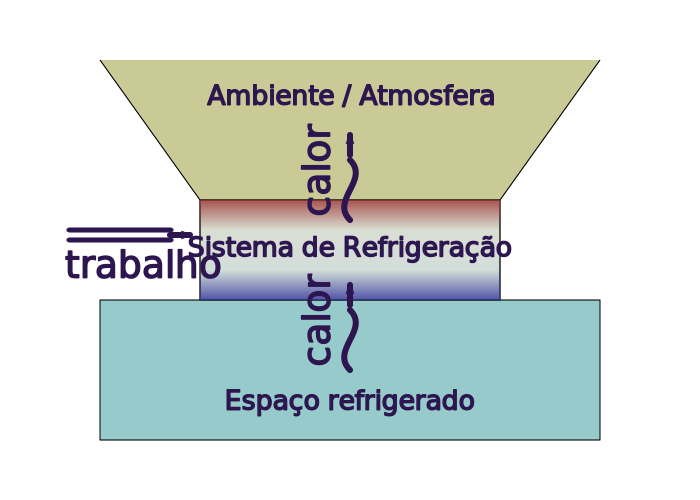
\includegraphics[height=0.8\textheight]{fig/01-SistemaRefrGen.pdf}
                    \\\vspace*{-1em}\texttt{autoria própria}
                \end{figure}
            \end{center}
            \vfill
		\end{columns}
    \end{frame}
    %-------------------------------------------------------------------------------------------

%-----------------------------------------------------------------------------------------------
\subsection{Classificação dos Sistemas}
%-----------------------------------------------------------------------------------------------

    % !j 96 -i8
    %-------------------------------------------------------------------------------------------
    \begin{frame}{Tipos de Sistemas de Refrigeração}\vspace*{-0em}
        Dentre os tipos de sistema de refrigeração, destaca-se: \\[\medskipamount]
        \begin{itemize}
            \item<1-> Sistemas de \alert{compressão de vapor};
            \item<2-> Sistemas à \alert{ar ou à gás};
            \item<3-> Sistemas de \alert{absorção};
            \item<4-> Sistemas \alert{termo-elétricos};
            \item<5-> Resfriadores \alert{evaporativos}.
        \end{itemize}
    \end{frame}
    %-------------------------------------------------------------------------------------------

    % !j 96 -i8
    %-------------------------------------------------------------------------------------------
    \begin{frame}{Sistemas por Compressão de Vapor}\vspace*{-0em}
        \begin{itemize}
            \item<1-> É o tipo atualmente \alert{mais comumente utilizado} na atualidade;
                \\[\medskipamount]
            \item<2-> O \alert{fluido de trabalho} de tais sistemas é chamado de
                \alert{refrigerante};
                \\[\medskipamount]
            \item<3-> Em tais ciclos os refrigerantes \alert{mudam de fase} entre
                \alert{líquido} e \alert{vapor};
                \\[\medskipamount]
            \item<4-> Os principais componentes são: \alert{evaporador}, \alert{compressor},
                \alert{condensador} e \alert{dispositivo de expansão};
                \\[\medskipamount]
            \item<5-> Um pequeno sistema (\alert{ciclo}) é ilustrado a seguir:
        \end{itemize}
    \end{frame}
    %-------------------------------------------------------------------------------------------
    \begin{frame}\vspace*{-0em}
        \begin{center}
            \begin{figure}
                \fontsize{5.0}{5}\selectfont
                \includegraphics[height=0.9\textheight]{ext/2016-FentonDL-Fig-1-2.jpg}
                \\\vspace*{-0.0em}\texttt{%
                    Sistema simples de refrigeração por compressão de vapor.\\
                    Fonte: referência~\cite{2016-FentonDL-ASHRAE}
                }
            \end{figure}
        \end{center}
    \end{frame}
    %-------------------------------------------------------------------------------------------

    %-------------------------------------------------------------------------------------------
    \begin{frame}\vspace*{-0em}
        \begin{center}
            \begin{figure}
                \fontsize{5.0}{5}\selectfont
                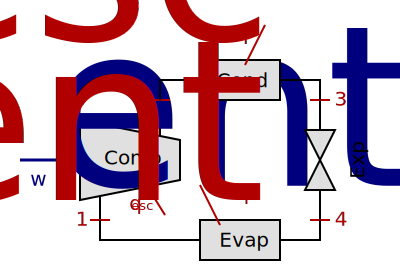
\includegraphics[height=0.9\textheight]{fig/0002-Refr-Vap-ID.pdf}
                \\\vspace*{-0.0em}\texttt{%
                    Esquemático de sistema de refrigeração por compressão de vapor.\\
                    Fonte: autoria própria
                }
            \end{figure}
        \end{center}
    \end{frame}
    %-------------------------------------------------------------------------------------------

    % !j 96 -i8
    %-------------------------------------------------------------------------------------------
    \begin{frame}{Sistemas a Ar (Gás)}\vspace*{-0em}
        \begin{itemize}
            \item<1-> O \alert{fluido de trabalho} de tais sistemas é um \alert{gás}, geralmente
                o \alert{ar};
            \item<2-> Nos sistemas a gás, o fluido de trabalho \alert{não muda de fase}, sendo
                sempre um gás;
            \item<3-> Processos incluem o de (i)~\alert{compressão} de ar, no qual a sua
                temperatura \alert{aumenta};
            \item<4-> (ii)~\alert{troca de calor} (sensível) para a atmosfera, no qual a sua temperatura \alert{diminui};
            \item<5-> (iii)~\alert{expansão} em um dispositivo que recupera \alert{trabalho},
                que provoca a \alert{redução} da temperatura do ar;
            \item<6-> (iv)~\alert{mistura} do ar expandido com aquele do espaço refrigerado, ou
                seja: \alert{injeção de ar frio} diretamente no espaço refrigerado.
            \item<7-> Sistemas e variantes são ilustrados a seguir:
        \end{itemize}
    \end{frame}
    %-------------------------------------------------------------------------------------------

    %-------------------------------------------------------------------------------------------
    \begin{frame}\vspace*{-0em}
        \begin{center}
            \begin{figure}
                \fontsize{5.0}{5}\selectfont
                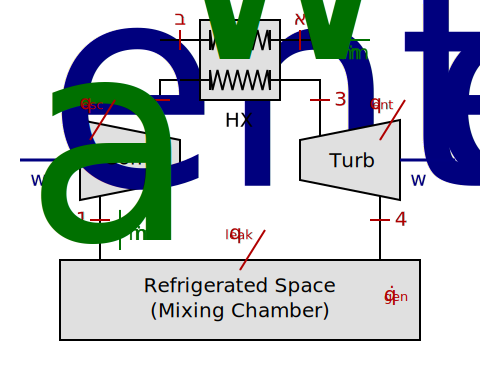
\includegraphics[height=0.9\textheight]{fig/0003-Comp+HX+Turb.pdf}
                \\\vspace*{-0.0em}\texttt{%
                    Esquemático de sistema de refrigeração a ar.\\
                    Fonte: autoria própria
                }
            \end{figure}
        \end{center}
    \end{frame}
    %-------------------------------------------------------------------------------------------

    % !j 96 -i8
    %-------------------------------------------------------------------------------------------
    \begin{frame}\vspace*{-0em}
        \wwwfigH{airplane-01}{jpg}{url}
    \end{frame}
    %-------------------------------------------------------------------------------------------

    % !j 96 -i8
    %-------------------------------------------------------------------------------------------
    \begin{frame}\vspace*{-0em}
        \wwwfigH{airplane-02}{jpg}{url}
    \end{frame}
    %-------------------------------------------------------------------------------------------

    % !j 96 -i8
    %-------------------------------------------------------------------------------------------
    \begin{frame}\vspace*{-0em}
        \wwwfigH{airplane-03}{jpg}{url}
    \end{frame}
    %-------------------------------------------------------------------------------------------

    % !j 96 -i8
    %-------------------------------------------------------------------------------------------
    \begin{frame}\vspace*{-0em}
        \wwwfigH{airplane-04}{jpg}{url}
    \end{frame}
    %-------------------------------------------------------------------------------------------

    % !j 96 -i8
    %-------------------------------------------------------------------------------------------
    \begin{frame}{Sistemas de Absorção}\vspace*{-0em}
        \begin{itemize}
            \item<1-> Sistemas de \alert{absorção} são semelhantes a sistemas a \alert{vapor};
                \\[\medskipamount]
            \item<2-> Porém, sistemas de absorção trocam \alert{compressão de gás} por
                \alert{bombeamento} de líquido;
                \\[\medskipamount]
            \item<3-> Isto evidentemente \alert{economiza trabalho};
                \\[\medskipamount]
            \item<4-> Porém exige \alert{fornecimentos e retiradas de calor} extras na
                \alert{absorção} e \alert{geração} do vapor;
                \\[\medskipamount]
            \item<5-> Tais sistemas utilizam fluidos \alert{refrigerante} e \alert{absorvente};
                \\[\medskipamount]
            \item<6-> Variantes \alert{mais comuns}: (i)~\alert{\ce{NH3} em \ce{H2O}} e
                (ii)~\alert{\ce{H2O} em \ce{LiBr}};
                \\[\medskipamount]
            \item<7-> Solubilidade do refrigerante no absorvente é \alert{função da
                temperatura}.
        \end{itemize}
    \end{frame}
    %-------------------------------------------------------------------------------------------
    \begin{frame}{Sistemas de Absorção -- Solubilidade de \ce{NH3} em \ce{H2O}}\vspace*{-0em}
        \begin{columns}
            \column{0.5\textwidth}
            \wwwfig{ammonia-01}{jpg}{yt}
            \column{0.5\textwidth}
            \wwwfig{ammonia-02}{jpg}{yt}
        \end{columns}
    \end{frame}
    %-------------------------------------------------------------------------------------------
    \begin{frame}{Sistemas de Absorção -- Solubilidade de \ce{NH3} em \ce{H2O}}\vspace*{-0em}
        \begin{columns}
            \column{0.5\textwidth}
            \wwwfig{ammonia-03}{jpg}{yt}
            \column{0.5\textwidth}
            \wwwfig{ammonia-04}{jpg}{yt}
        \end{columns}
    \end{frame}
    %-------------------------------------------------------------------------------------------
    \begin{frame}\vspace*{-0em}
        \begin{center}
            \begin{figure}
                \fontsize{5.0}{5}\selectfont
                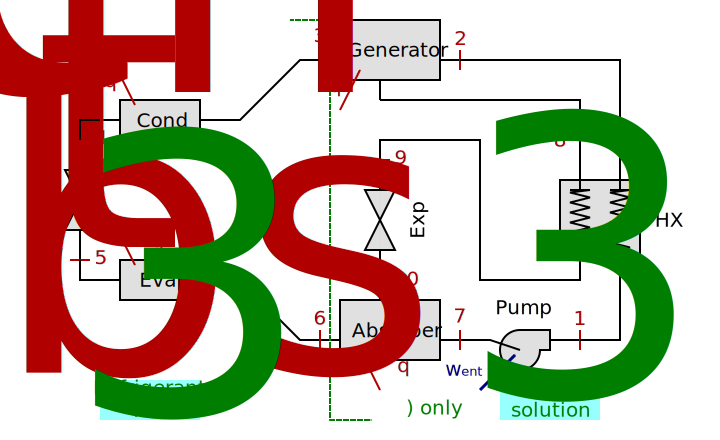
\includegraphics[height=0.9\textheight]{fig/0004-Absorpt-Refr-H2O+NH3.pdf}
                \\\vspace*{-0.0em}\texttt{%
                    Esquemático de sistema de refrigeração por absorção Água-Amônia.\\
                    Fonte: autoria própria
                }
            \end{figure}
        \end{center}
    \end{frame}
    %-------------------------------------------------------------------------------------------
    \begin{frame}\vspace*{-0em}
        \begin{center}
            \begin{figure}
                \fontsize{5.0}{5}\selectfont
                \includegraphics[height=0.9\textheight]{ext/1993-PetersR+KellerJU-Table-1.png}
                \\\vspace*{-0.0em}\texttt{%
                    Sistema simples de refrigeração por compressão de vapor.\\
                    Fonte: referência~\cite{1993-PetersR+KellerJU-IntjThermoPhys}
                }
            \end{figure}
        \end{center}
    \end{frame}
    %-------------------------------------------------------------------------------------------
    \begin{frame}\vspace*{-0em}
        \begin{center}
            \begin{figure}
                \fontsize{5.0}{5}\selectfont
                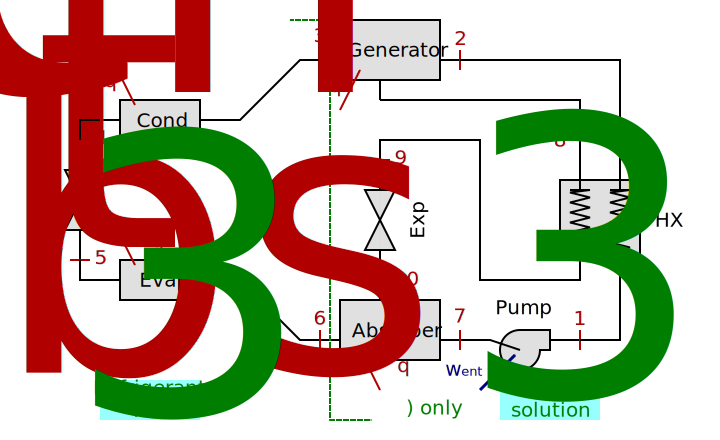
\includegraphics[height=0.9\textheight]{fig/0005-Absorpt-Refr-BrLi+H2O.pdf}
                \\\vspace*{-0.0em}\texttt{%
                    Esquemático de sistema de refrigeração por absorção Brometo de Lítio-Água.
                    Ciclos em chillers industriais podem diferir significativamente com a
                    tecnologia de cada fabricante.\\
                    Fonte: autoria própria
                }
            \end{figure}
        \end{center}
    \end{frame}
    %-------------------------------------------------------------------------------------------
    \begin{frame}\vspace*{-0em}
        \wwwfigH{16DJ-Absorption-Chiller}{jpg}{url}
    \end{frame}
    %-------------------------------------------------------------------------------------------
    \begin{frame}\vspace*{-0em}
        \begin{center}
            \begin{figure}
                \fontsize{5.0}{5}\selectfont
                \includegraphics[height=0.9\textheight]{ext/PSD-16DJ_11-82-Fig-1.pdf}
                \\\vspace*{-0.0em}\texttt{%
                    Ciclo de absorção LiBr-água simplificado.\\
                   Fonte: \input{ext/PSD-16DJ_11-82-Fig-1.url}
                }
            \end{figure}
        \end{center}
    \end{frame}
    %-------------------------------------------------------------------------------------------

    % !j 96 -i8
    %-------------------------------------------------------------------------------------------
    \begin{frame}{Sistemas Termo-Elétricos}\vspace*{-0em}
        \begin{itemize}
            \item<1-> Exploram o \alert{efeito Peltier};
                \\[\medskipamount]
            \item<2-> Resfriamento e aquecimento de junções \alert{semicondutoras} dissimilares;
                \\[\medskipamount]
            \item<3-> Pela passagem de corrente elétrica, i.e., \alert{trabalho elétrico}.
                \\[\medskipamount]
            \item<4-> Superfície fria pode \alert{absorver calor} do espaço refrigerado;
                \\[\medskipamount]
            \item<5-> Superfície aquecida pode \alert{transferir calor} ao ambiente;
                \\[\medskipamount]
            \item<6-> Sistemas \alert{práticos} utilizam juntas semicondutoras em série
                ($\uparrow\Delta{T}$).
        \end{itemize}
    \end{frame}
    %-------------------------------------------------------------------------------------------
    \begin{frame}\vspace*{-0em}
        \begin{center}
            \begin{figure}
                \fontsize{5.0}{5}\selectfont
                \includegraphics[height=0.9\textheight]{ext/2016-FentonDL-Fig-1-5.jpg}
                \\\vspace*{-0.0em}\texttt{%
                    Sistema simples de refrigeração por compressão de vapor.\\
                    Fonte: referência~\cite{2016-FentonDL-ASHRAE}
                }
            \end{figure}
        \end{center}
    \end{frame}
    %-------------------------------------------------------------------------------------------
    \begin{frame}\vspace*{-0em}
        \wwwfigH{thermoelectric-01}{jpg}{short}
    \end{frame}
    %-------------------------------------------------------------------------------------------
    \begin{frame}\vspace*{-0em}
        \wwwfigH{thermoelectric-02}{jpg}{short}
    \end{frame}
    %-------------------------------------------------------------------------------------------
    \begin{frame}\vspace*{-0em}
        \begin{columns}
            \column{0.5\textwidth}
            \wwwfigH{thermoelectric-03}{jpg}{short}
            \column{0.5\textwidth}
            \wwwfigH{thermoelectric-04}{jpg}{short}
        \end{columns}
    \end{frame}
    %-------------------------------------------------------------------------------------------
    \begin{frame}\vspace*{-0em}
        \begin{columns}
            \column{0.5\textwidth}
            \wwwfigH{thermoelectric-05}{jpg}{short}
            \column{0.5\textwidth}
            \wwwfigH{thermoelectric-06}{jpg}{short}
        \end{columns}
    \end{frame}
    %-------------------------------------------------------------------------------------------

    % !j 96 -i8
    %-------------------------------------------------------------------------------------------
    \begin{frame}{Resfriadores Evaporativos}\vspace*{-0em}
        \begin{columns}
        \column{0.55\textwidth}
            Coluna com 55\% de largura:\\[\smallskipamount]
            \begin{itemize}
                \item<1-> Item 1;
                \item<2-> Item 2;
                \item<3-> Item 3.
            \end{itemize}
        \column{0.45\textwidth}
            Coluna com 45\% de largura.
            \begin{center}
                \begin{figure}
                    \includegraphics[width=0.5\textwidth]{www/moringa-01.jpg}
                \end{figure}
            \end{center}
        \end{columns}
    \end{frame}
    %-------------------------------------------------------------------------------------------

%-----------------------------------------------------------------------------------------------
\subsection{Processos de Refrigeração}
%-----------------------------------------------------------------------------------------------

    % !j 96 -i8
    %-------------------------------------------------------------------------------------------
    \begin{frame}{Ciclo de Refrigeração por Compressão de Vapor}\vspace*{-0em}
        \begin{itemize}
            \item<1-> Definições;
            \item<1-> Item 2;
            \item<1-> Item 3.
        \end{itemize}
    \end{frame}
    %-------------------------------------------------------------------------------------------

    % !j 96 -i8
    %-------------------------------------------------------------------------------------------
    \begin{frame}{Ciclo Bomba de Calor}\vspace*{-0em}
        \begin{itemize}
            \item<1-> Definições;
            \item<1-> Item 2;
            \item<1-> Item 3.
        \end{itemize}
    \end{frame}
    %-------------------------------------------------------------------------------------------

%-----------------------------------------------------------------------------------------------
\section{Aplicações de Refrigeração}
%-----------------------------------------------------------------------------------------------

%-----------------------------------------------------------------------------------------------
\subsection{Classificação por Capacidade}
%-----------------------------------------------------------------------------------------------

    % !j 96 -i8
    %-------------------------------------------------------------------------------------------
    \begin{frame}{O Ramo de Refrigeração}\vspace*{-0em}
        \begin{itemize}
            \item<1-> Doméstico, \alert{menos de $\unit{20}{\kilo\watt}$};
            \item<2-> Comercial, \alert{mais de $\unit{20}{\kilo\watt}$};
            \item<3-> Industrial, \alert{de pequeno a muito grande}.
        \end{itemize}
    \end{frame}
    %-------------------------------------------------------------------------------------------

%-----------------------------------------------------------------------------------------------
\subsection{Classificação por Aplicação}
%-----------------------------------------------------------------------------------------------

    % !j 96 -i8
    %-------------------------------------------------------------------------------------------
    \begin{frame}{Aplicações de Refrigeração}\vspace*{-0em}
        \begin{itemize}
            \item<1-> Condicionamento de ar residencial;
            \item<2-> Condicionamento de ar veicular;
            \item<3-> Condicionamento de ar de médios e grandes edificações;
            \item<4-> Transporte de cargas;
            \item<5-> Refrigeração residencial;
            \item<6-> Refrigeração de máquinas de venda;
            \item<7-> Ar-condicionado industrial;
            \item<8-> Refrigeração industrial;
        \end{itemize}
    \end{frame}
    %-------------------------------------------------------------------------------------------

    % !j 96 -i8
    %-------------------------------------------------------------------------------------------
    \begin{frame}{Ar-condicionado Industrial}\vspace*{-0em}
        \begin{itemize}
            \item<1-> Item 1;
            \item<2-> Item 2;
            \item<3-> Item 3.
        \end{itemize}
    \end{frame}
    %-------------------------------------------------------------------------------------------

    % !j 96 -i8
    %-------------------------------------------------------------------------------------------
    \begin{frame}{Refrigeração Industrial}\vspace*{-0em}
        \begin{itemize}
            \item<1-> Item 1;
            \item<2-> Item 2;
            \item<3-> Item 3.
        \end{itemize}
    \end{frame}
    %-------------------------------------------------------------------------------------------

%-----------------------------------------------------------------------------------------------
\section{Referências e Tópicos de Leitura}
%-----------------------------------------------------------------------------------------------

    %------------------------------------------------------------------------------------------
    \begin{frame}[allowframebreaks]{Referências -- }
        \bibliographystyle{unsrt}
        \setbeamertemplate{bibliography item}{\insertbiblabel}
        \bibliography{bibfile.bib}
    \end{frame}
    %------------------------------------------------------------------------------------------

    % Finishes with stunning image, with credit
    \ArtEndWSE{pexels-pixabay-207985}{jpg}{txt}

%-----------------------------------------------------------------------------------------------
\end{document}
%-----------------------------------------------------------------------------------------------

